\documentclass[1p]{elsarticle_modified}
%\bibliographystyle{elsarticle-num}

%\usepackage[colorlinks]{hyperref}
%\usepackage{abbrmath_seonhwa} %\Abb, \Ascr, \Acal ,\Abf, \Afrak
\usepackage{amsfonts}
\usepackage{amssymb}
\usepackage{amsmath}
\usepackage{amsthm}
\usepackage{scalefnt}
\usepackage{amsbsy}
\usepackage{kotex}
\usepackage{caption}
\usepackage{subfig}
\usepackage{color}
\usepackage{graphicx}
\usepackage{xcolor} %% white, black, red, green, blue, cyan, magenta, yellow
\usepackage{float}
\usepackage{setspace}
\usepackage{hyperref}

\usepackage{tikz}
\usetikzlibrary{arrows}

\usepackage{multirow}
\usepackage{array} % fixed length table
\usepackage{hhline}

%%%%%%%%%%%%%%%%%%%%%
\makeatletter
\renewcommand*\env@matrix[1][\arraystretch]{%
	\edef\arraystretch{#1}%
	\hskip -\arraycolsep
	\let\@ifnextchar\new@ifnextchar
	\array{*\c@MaxMatrixCols c}}
\makeatother %https://tex.stackexchange.com/questions/14071/how-can-i-increase-the-line-spacing-in-a-matrix
%%%%%%%%%%%%%%%

\usepackage[normalem]{ulem}

\newcommand{\msout}[1]{\ifmmode\text{\sout{\ensuremath{#1}}}\else\sout{#1}\fi}
%SOURCE: \msout is \stkout macro in https://tex.stackexchange.com/questions/20609/strikeout-in-math-mode

\newcommand{\cancel}[1]{
	\ifmmode
	{\color{red}\msout{#1}}
	\else
	{\color{red}\sout{#1}}
	\fi
}

\newcommand{\add}[1]{
	{\color{blue}\uwave{#1}}
}

\newcommand{\replace}[2]{
	\ifmmode
	{\color{red}\msout{#1}}{\color{blue}\uwave{#2}}
	\else
	{\color{red}\sout{#1}}{\color{blue}\uwave{#2}}
	\fi
}

\newcommand{\Sol}{\mathcal{S}} %segment
\newcommand{\D}{D} %diagram
\newcommand{\A}{\mathcal{A}} %arc


%%%%%%%%%%%%%%%%%%%%%%%%%%%%%5 test

\def\sl{\operatorname{\textup{SL}}(2,\Cbb)}
\def\psl{\operatorname{\textup{PSL}}(2,\Cbb)}
\def\quan{\mkern 1mu \triangleright \mkern 1mu}

\theoremstyle{definition}
\newtheorem{thm}{Theorem}[section]
\newtheorem{prop}[thm]{Proposition}
\newtheorem{lem}[thm]{Lemma}
\newtheorem{ques}[thm]{Question}
\newtheorem{cor}[thm]{Corollary}
\newtheorem{defn}[thm]{Definition}
\newtheorem{exam}[thm]{Example}
\newtheorem{rmk}[thm]{Remark}
\newtheorem{alg}[thm]{Algorithm}

\newcommand{\I}{\sqrt{-1}}
\begin{document}

%\begin{frontmatter}
%
%\title{Boundary parabolic representations of knots up to 8 crossings}
%
%%% Group authors per affiliation:
%\author{Yunhi Cho} 
%\address{Department of Mathematics, University of Seoul, Seoul, Korea}
%\ead{yhcho@uos.ac.kr}
%
%
%\author{Seonhwa Kim} %\fnref{s_kim}}
%\address{Center for Geometry and Physics, Institute for Basic Science, Pohang, 37673, Korea}
%\ead{ryeona17@ibs.re.kr}
%
%\author{Hyuk Kim}
%\address{Department of Mathematical Sciences, Seoul National University, Seoul 08826, Korea}
%\ead{hyukkim@snu.ac.kr}
%
%\author{Seokbeom Yoon}
%\address{Department of Mathematical Sciences, Seoul National University, Seoul, 08826,  Korea}
%\ead{sbyoon15@snu.ac.kr}
%
%\begin{abstract}
%We find all boundary parabolic representation of knots up to 8 crossings.
%
%\end{abstract}
%\begin{keyword}
%    \MSC[2010] 57M25 
%\end{keyword}
%
%\end{frontmatter}

%\linenumbers
%\tableofcontents
%
\newcommand\colored[1]{\textcolor{white}{\rule[-0.35ex]{0.8em}{1.4ex}}\kern-0.8em\color{red} #1}%
%\newcommand\colored[1]{\textcolor{white}{ #1}\kern-2.17ex	\textcolor{white}{ #1}\kern-1.81ex	\textcolor{white}{ #1}\kern-2.15ex\color{red}#1	}

{\Large $\underline{12n_{0144}~(K12n_{0144})}$}

\setlength{\tabcolsep}{10pt}
\renewcommand{\arraystretch}{1.6}
\vspace{1cm}\begin{tabular}{m{100pt}>{\centering\arraybackslash}m{274pt}}
\multirow{5}{120pt}{
	\centering
	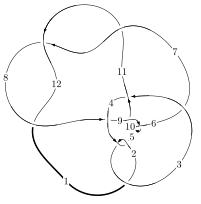
\includegraphics[width=112pt]{../../../GIT/diagram.site/Diagrams/png/2233_12n_0144.png}\\
\ \ \ A knot diagram\footnotemark}&
\allowdisplaybreaks
\textbf{Linearized knot diagam} \\
\cline{2-2}
 &
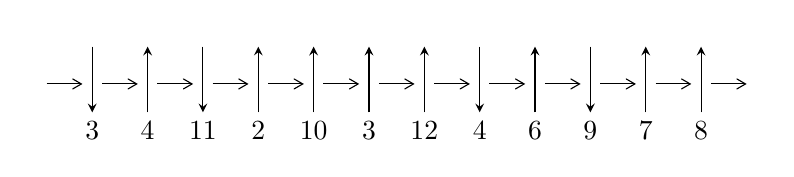
\begin{tikzpicture}[x=20pt, y=17pt]
	% nodes
	\node (C0) at (0, 0) {};
	\node (C1) at (1, 0) {};
	\node (C1U) at (1, +1) {};
	\node (C1D) at (1, -1) {3};

	\node (C2) at (2, 0) {};
	\node (C2U) at (2, +1) {};
	\node (C2D) at (2, -1) {4};

	\node (C3) at (3, 0) {};
	\node (C3U) at (3, +1) {};
	\node (C3D) at (3, -1) {11};

	\node (C4) at (4, 0) {};
	\node (C4U) at (4, +1) {};
	\node (C4D) at (4, -1) {2};

	\node (C5) at (5, 0) {};
	\node (C5U) at (5, +1) {};
	\node (C5D) at (5, -1) {10};

	\node (C6) at (6, 0) {};
	\node (C6U) at (6, +1) {};
	\node (C6D) at (6, -1) {3};

	\node (C7) at (7, 0) {};
	\node (C7U) at (7, +1) {};
	\node (C7D) at (7, -1) {12};

	\node (C8) at (8, 0) {};
	\node (C8U) at (8, +1) {};
	\node (C8D) at (8, -1) {4};

	\node (C9) at (9, 0) {};
	\node (C9U) at (9, +1) {};
	\node (C9D) at (9, -1) {6};

	\node (C10) at (10, 0) {};
	\node (C10U) at (10, +1) {};
	\node (C10D) at (10, -1) {9};

	\node (C11) at (11, 0) {};
	\node (C11U) at (11, +1) {};
	\node (C11D) at (11, -1) {7};

	\node (C12) at (12, 0) {};
	\node (C12U) at (12, +1) {};
	\node (C12D) at (12, -1) {8};
	\node (C13) at (13, 0) {};

	% arrows
	\draw[->,>={angle 60}]
	(C0) edge (C1) (C1) edge (C2) (C2) edge (C3) (C3) edge (C4) (C4) edge (C5) (C5) edge (C6) (C6) edge (C7) (C7) edge (C8) (C8) edge (C9) (C9) edge (C10) (C10) edge (C11) (C11) edge (C12) (C12) edge (C13) ;	\draw[->,>=stealth]
	(C1U) edge (C1D) (C2D) edge (C2U) (C3U) edge (C3D) (C4D) edge (C4U) (C5D) edge (C5U) (C6D) edge (C6U) (C7D) edge (C7U) (C8U) edge (C8D) (C9D) edge (C9U) (C10U) edge (C10D) (C11D) edge (C11U) (C12D) edge (C12U) ;
	\end{tikzpicture} \\
\hhline{~~} \\& 
\textbf{Solving Sequence} \\ \cline{2-2} 
 &
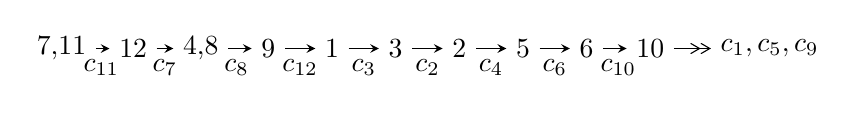
\begin{tikzpicture}[x=23pt, y=7pt]
	% node
	\node (A0) at (-1/8, 0) {7,11};
	\node (A1) at (1, 0) {12};
	\node (A2) at (33/16, 0) {4,8};
	\node (A3) at (25/8, 0) {9};
	\node (A4) at (33/8, 0) {1};
	\node (A5) at (41/8, 0) {3};
	\node (A6) at (49/8, 0) {2};
	\node (A7) at (57/8, 0) {5};
	\node (A8) at (65/8, 0) {6};
	\node (A9) at (73/8, 0) {10};
	\node (C1) at (1/2, -1) {$c_{11}$};
	\node (C2) at (3/2, -1) {$c_{7}$};
	\node (C3) at (21/8, -1) {$c_{8}$};
	\node (C4) at (29/8, -1) {$c_{12}$};
	\node (C5) at (37/8, -1) {$c_{3}$};
	\node (C6) at (45/8, -1) {$c_{2}$};
	\node (C7) at (53/8, -1) {$c_{4}$};
	\node (C8) at (61/8, -1) {$c_{6}$};
	\node (C9) at (69/8, -1) {$c_{10}$};
	\node (A10) at (11, 0) {$c_{1},c_{5},c_{9}$};

	% edge
	\draw[->,>=stealth]	
	(A0) edge (A1) (A1) edge (A2) (A2) edge (A3) (A3) edge (A4) (A4) edge (A5) (A5) edge (A6) (A6) edge (A7) (A7) edge (A8) (A8) edge (A9) ;
	\draw[->>,>={angle 60}]	
	(A9) edge (A10);
\end{tikzpicture} \\ 

\end{tabular} \\

\footnotetext{
The image of knot diagram is generated by the software ``\textbf{Draw programme}" developed by Andrew Bartholomew(\url{http://www.layer8.co.uk/maths/draw/index.htm\#Running-draw}), where we modified some parts for our purpose(\url{https://github.com/CATsTAILs/LinksPainter}).
}\phantom \\ \newline 
\centering \textbf{Ideals for irreducible components\footnotemark of $X_{\text{par}}$} 
 
\begin{align*}
I^u_{1}&=\langle 
7.34372\times10^{20} u^{43}+1.60104\times10^{21} u^{42}+\cdots+6.28525\times10^{21} b+5.02483\times10^{21},\\
\phantom{I^u_{1}}&\phantom{= \langle  }1.42649\times10^{20} u^{43}+6.11830\times10^{20} u^{42}+\cdots+3.14262\times10^{21} a-1.33924\times10^{20},\;u^{44}+4 u^{43}+\cdots+32 u+16\rangle \\
I^u_{2}&=\langle 
4 b+2 a- u+2,\;2 a^2-2 a u+7,\;u^2-2\rangle \\
I^u_{3}&=\langle 
a u+7 b+4 a+u+4,\;2 a^2+a u-3 u+7,\;u^2-2\rangle \\
I^u_{4}&=\langle 
3 a^4-4 a^3+24 a^2+2 b-25 a+8,\;a^5-2 a^4+9 a^3-14 a^2+9 a-2,\;u-1\rangle \\
\\
I^v_{1}&=\langle 
a,\;b- v-1,\;v^2+v+1\rangle \\
I^v_{2}&=\langle 
a,\;b^2- b+1,\;v-1\rangle \\
\end{align*}
\raggedright * 6 irreducible components of $\dim_{\mathbb{C}}=0$, with total 61 representations.\\
\footnotetext{All coefficients of polynomials are rational numbers. But the coefficients are sometimes approximated in decimal forms when there is not enough margin.}
\newpage
\renewcommand{\arraystretch}{1}
\centering \section*{I. $I^u_{1}= \langle 7.34\times10^{20} u^{43}+1.60\times10^{21} u^{42}+\cdots+6.29\times10^{21} b+5.02\times10^{21},\;1.43\times10^{20} u^{43}+6.12\times10^{20} u^{42}+\cdots+3.14\times10^{21} a-1.34\times10^{20},\;u^{44}+4 u^{43}+\cdots+32 u+16 \rangle$}
\flushleft \textbf{(i) Arc colorings}\\
\begin{tabular}{m{7pt} m{180pt} m{7pt} m{180pt} }
\flushright $a_{7}=$&$\begin{pmatrix}0\\u\end{pmatrix}$ \\
\flushright $a_{11}=$&$\begin{pmatrix}1\\0\end{pmatrix}$ \\
\flushright $a_{12}=$&$\begin{pmatrix}1\\- u^2\end{pmatrix}$ \\
\flushright $a_{4}=$&$\begin{pmatrix}-0.0453917 u^{43}-0.194688 u^{42}+\cdots-0.0781355 u+0.0426155\\-0.116841 u^{43}-0.254730 u^{42}+\cdots-2.09430 u-0.799464\end{pmatrix}$ \\
\flushright $a_{8}=$&$\begin{pmatrix}u\\- u^3+u\end{pmatrix}$ \\
\flushright $a_{9}=$&$\begin{pmatrix}0.191388 u^{43}+0.550760 u^{42}+\cdots+3.38008 u+3.58656\\-0.0541941 u^{43}-0.188082 u^{42}+\cdots-0.273250 u-1.13238\end{pmatrix}$ \\
\flushright $a_{1}=$&$\begin{pmatrix}- u^2+1\\u^4-2 u^2\end{pmatrix}$ \\
\flushright $a_{3}=$&$\begin{pmatrix}-0.162232 u^{43}-0.449417 u^{42}+\cdots-2.17243 u-0.756849\\-0.116841 u^{43}-0.254730 u^{42}+\cdots-2.09430 u-0.799464\end{pmatrix}$ \\
\flushright $a_{2}=$&$\begin{pmatrix}-0.459894 u^{43}-1.20645 u^{42}+\cdots-7.93846 u-3.69776\\0.319896 u^{43}+0.993797 u^{42}+\cdots+4.40818 u+5.01424\end{pmatrix}$ \\
\flushright $a_{5}=$&$\begin{pmatrix}0.873473 u^{43}+2.49705 u^{42}+\cdots+13.0049 u+12.6274\\u^4-2 u^2\end{pmatrix}$ \\
\flushright $a_{6}=$&$\begin{pmatrix}-0.776380 u^{43}-2.07570 u^{42}+\cdots-12.3449 u-8.51440\\0.297158 u^{43}+0.926397 u^{42}+\cdots+6.35873 u+4.85216\end{pmatrix}$ \\
\flushright $a_{10}=$&$\begin{pmatrix}-0.335109 u^{43}-1.04952 u^{42}+\cdots-6.89963 u-4.51774\\-0.185846 u^{43}-0.499407 u^{42}+\cdots-2.65438 u-1.59651\end{pmatrix}$\\&\end{tabular}
\flushleft \textbf{(ii) Obstruction class $= -1$}\\~\\
\flushleft \textbf{(iii) Cusp Shapes $= \frac{1752784223058518261005}{785655665183033765648} u^{43}+\frac{2500993104539143938499}{392827832591516882824} u^{42}+\cdots+\frac{1124081559828742593975}{49103479073939610353} u+\frac{1641699334520185355340}{49103479073939610353}$}\\~\\
\newpage\renewcommand{\arraystretch}{1}
\flushleft \textbf{(iv) u-Polynomials at the component}\newline \\
\begin{tabular}{m{50pt}|m{274pt}}
Crossings & \hspace{64pt}u-Polynomials at each crossing \\
\hline $$\begin{aligned}c_{1}\end{aligned}$$&$\begin{aligned}
&u^{44}+51 u^{43}+\cdots-38168 u+2401
\end{aligned}$\\
\hline $$\begin{aligned}c_{2},c_{4}\end{aligned}$$&$\begin{aligned}
&u^{44}-11 u^{43}+\cdots-796 u+49
\end{aligned}$\\
\hline $$\begin{aligned}c_{3}\end{aligned}$$&$\begin{aligned}
&u^{44}+3 u^{43}+\cdots-4 u+7
\end{aligned}$\\
\hline $$\begin{aligned}c_{5},c_{9}\end{aligned}$$&$\begin{aligned}
&u^{44}-3 u^{43}+\cdots-14 u+7
\end{aligned}$\\
\hline $$\begin{aligned}c_{6}\end{aligned}$$&$\begin{aligned}
&u^{44}+2 u^{43}+\cdots-7517 u+13159
\end{aligned}$\\
\hline $$\begin{aligned}c_{7},c_{11},c_{12}\end{aligned}$$&$\begin{aligned}
&u^{44}+4 u^{43}+\cdots+32 u+16
\end{aligned}$\\
\hline $$\begin{aligned}c_{8}\end{aligned}$$&$\begin{aligned}
&u^{44}-2 u^{43}+\cdots-23256067 u+7050439
\end{aligned}$\\
\hline $$\begin{aligned}c_{10}\end{aligned}$$&$\begin{aligned}
&u^{44}+27 u^{43}+\cdots+476 u+49
\end{aligned}$\\
\hline
\end{tabular}\\~\\
\newpage\renewcommand{\arraystretch}{1}
\flushleft \textbf{(v) Riley Polynomials at the component}\newline \\
\begin{tabular}{m{50pt}|m{274pt}}
Crossings & \hspace{64pt}Riley Polynomials at each crossing \\
\hline $$\begin{aligned}c_{1}\end{aligned}$$&$\begin{aligned}
&y^{44}-109 y^{43}+\cdots-778696200 y+5764801
\end{aligned}$\\
\hline $$\begin{aligned}c_{2},c_{4}\end{aligned}$$&$\begin{aligned}
&y^{44}+51 y^{43}+\cdots-38168 y+2401
\end{aligned}$\\
\hline $$\begin{aligned}c_{3}\end{aligned}$$&$\begin{aligned}
&y^{44}+11 y^{43}+\cdots+796 y+49
\end{aligned}$\\
\hline $$\begin{aligned}c_{5},c_{9}\end{aligned}$$&$\begin{aligned}
&y^{44}+27 y^{43}+\cdots+476 y+49
\end{aligned}$\\
\hline $$\begin{aligned}c_{6}\end{aligned}$$&$\begin{aligned}
&y^{44}+26 y^{43}+\cdots+5158564319 y+173159281
\end{aligned}$\\
\hline $$\begin{aligned}c_{7},c_{11},c_{12}\end{aligned}$$&$\begin{aligned}
&y^{44}-36 y^{43}+\cdots+1024 y+256
\end{aligned}$\\
\hline $$\begin{aligned}c_{8}\end{aligned}$$&$\begin{aligned}
&y^{44}-50 y^{43}+\cdots-570620658530165 y+49708690092721
\end{aligned}$\\
\hline $$\begin{aligned}c_{10}\end{aligned}$$&$\begin{aligned}
&y^{44}-13 y^{43}+\cdots+67816 y+2401
\end{aligned}$\\
\hline
\end{tabular}\\~\\
\newpage\flushleft \textbf{(vi) Complex Volumes and Cusp Shapes}
$$\begin{array}{c|c|c}  
\text{Solutions to }I^u_{1}& \I (\text{vol} + \sqrt{-1}CS) & \text{Cusp shape}\\
 \hline 
\begin{aligned}
u &= \phantom{-}0.053172 + 0.977197 I \\
a &= -0.726530 - 0.386151 I \\
b &= -0.881310 + 0.926174 I\end{aligned}
 & -7.21788 + 3.26048 I & \phantom{-}2.64523 - 2.48280 I \\ \hline\begin{aligned}
u &= \phantom{-}0.053172 - 0.977197 I \\
a &= -0.726530 + 0.386151 I \\
b &= -0.881310 - 0.926174 I\end{aligned}
 & -7.21788 - 3.26048 I & \phantom{-}2.64523 + 2.48280 I \\ \hline\begin{aligned}
u &= -0.969991 + 0.414842 I \\
a &= \phantom{-}0.607490 + 0.368276 I \\
b &= -0.799478 + 0.075673 I\end{aligned}
 & -1.73925 - 3.53680 I & \phantom{-}0.98095 + 4.14861 I \\ \hline\begin{aligned}
u &= -0.969991 - 0.414842 I \\
a &= \phantom{-}0.607490 - 0.368276 I \\
b &= -0.799478 - 0.075673 I\end{aligned}
 & -1.73925 + 3.53680 I & \phantom{-}0.98095 - 4.14861 I \\ \hline\begin{aligned}
u &= -0.174827 + 1.043030 I \\
a &= -0.718830 + 0.754972 I \\
b &= -0.888329 - 1.005910 I\end{aligned}
 & -11.08430 - 8.59782 I & \phantom{-}0.28005 + 5.55448 I \\ \hline\begin{aligned}
u &= -0.174827 - 1.043030 I \\
a &= -0.718830 - 0.754972 I \\
b &= -0.888329 + 1.005910 I\end{aligned}
 & -11.08430 + 8.59782 I & \phantom{-}0.28005 - 5.55448 I \\ \hline\begin{aligned}
u &= \phantom{-}0.074358 + 1.061190 I \\
a &= -0.353302 + 0.278439 I \\
b &= -0.957730 - 0.874395 I\end{aligned}
 & -11.51210 + 1.82027 I & -0.464174 - 0.761806 I \\ \hline\begin{aligned}
u &= \phantom{-}0.074358 - 1.061190 I \\
a &= -0.353302 - 0.278439 I \\
b &= -0.957730 + 0.874395 I\end{aligned}
 & -11.51210 - 1.82027 I & -0.464174 + 0.761806 I \\ \hline\begin{aligned}
u &= -1.060920 + 0.195318 I \\
a &= \phantom{-}0.943353 - 0.723894 I \\
b &= \phantom{-}0.729269 + 0.856189 I\end{aligned}
 & \phantom{-}1.66107 - 5.45145 I & \phantom{-}5.86619 + 6.59616 I \\ \hline\begin{aligned}
u &= -1.060920 - 0.195318 I \\
a &= \phantom{-}0.943353 + 0.723894 I \\
b &= \phantom{-}0.729269 - 0.856189 I\end{aligned}
 & \phantom{-}1.66107 + 5.45145 I & \phantom{-}5.86619 - 6.59616 I\\
 \hline 
 \end{array}$$\newpage$$\begin{array}{c|c|c}  
\text{Solutions to }I^u_{1}& \I (\text{vol} + \sqrt{-1}CS) & \text{Cusp shape}\\
 \hline 
\begin{aligned}
u &= -0.396864 + 0.675816 I \\
a &= \phantom{-}0.320038 - 0.485056 I \\
b &= \phantom{-}0.767519 + 0.420310 I\end{aligned}
 & -3.41945 - 0.63164 I & -2.08485 + 2.40121 I \\ \hline\begin{aligned}
u &= -0.396864 - 0.675816 I \\
a &= \phantom{-}0.320038 + 0.485056 I \\
b &= \phantom{-}0.767519 - 0.420310 I\end{aligned}
 & -3.41945 + 0.63164 I & -2.08485 - 2.40121 I \\ \hline\begin{aligned}
u &= \phantom{-}1.209100 + 0.327502 I \\
a &= -0.52561 - 2.57152 I \\
b &= -0.313533 + 1.159410 I\end{aligned}
 & \phantom{-}1.94616 + 7.53567 I & \phantom{-}4.00000 - 7.30881 I \\ \hline\begin{aligned}
u &= \phantom{-}1.209100 - 0.327502 I \\
a &= -0.52561 + 2.57152 I \\
b &= -0.313533 - 1.159410 I\end{aligned}
 & \phantom{-}1.94616 - 7.53567 I & \phantom{-}4.00000 + 7.30881 I \\ \hline\begin{aligned}
u &= -1.244840 + 0.163819 I \\
a &= -0.40678 + 2.39610 I \\
b &= -0.306940 - 1.055000 I\end{aligned}
 & \phantom{-}4.81580 - 3.31538 I & \phantom{-}11.03880 + 4.12292 I \\ \hline\begin{aligned}
u &= -1.244840 - 0.163819 I \\
a &= -0.40678 - 2.39610 I \\
b &= -0.306940 + 1.055000 I\end{aligned}
 & \phantom{-}4.81580 + 3.31538 I & \phantom{-}11.03880 - 4.12292 I \\ \hline\begin{aligned}
u &= -1.193050 + 0.633879 I \\
a &= -0.488351 + 0.504147 I \\
b &= \phantom{-}0.926853 - 0.905761 I\end{aligned}
 & -7.99420 + 2.74053 I & \phantom{-0.000000 } 0 \\ \hline\begin{aligned}
u &= -1.193050 - 0.633879 I \\
a &= -0.488351 - 0.504147 I \\
b &= \phantom{-}0.926853 + 0.905761 I\end{aligned}
 & -7.99420 - 2.74053 I & \phantom{-0.000000 } 0 \\ \hline\begin{aligned}
u &= \phantom{-}1.277500 + 0.501120 I \\
a &= -0.535158 - 0.270801 I \\
b &= \phantom{-}0.908252 + 0.813085 I\end{aligned}
 & -3.43084 + 1.99299 I & \phantom{-0.000000 } 0 \\ \hline\begin{aligned}
u &= \phantom{-}1.277500 - 0.501120 I \\
a &= -0.535158 + 0.270801 I \\
b &= \phantom{-}0.908252 - 0.813085 I\end{aligned}
 & -3.43084 - 1.99299 I & \phantom{-0.000000 } 0\\
 \hline 
 \end{array}$$\newpage$$\begin{array}{c|c|c}  
\text{Solutions to }I^u_{1}& \I (\text{vol} + \sqrt{-1}CS) & \text{Cusp shape}\\
 \hline 
\begin{aligned}
u &= \phantom{-}0.155102 + 0.599275 I \\
a &= \phantom{-}0.352478 - 1.113320 I \\
b &= \phantom{-}0.478851 + 1.053130 I\end{aligned}
 & -1.29319 - 4.02132 I & -0.30638 + 3.65044 I \\ \hline\begin{aligned}
u &= \phantom{-}0.155102 - 0.599275 I \\
a &= \phantom{-}0.352478 + 1.113320 I \\
b &= \phantom{-}0.478851 - 1.053130 I\end{aligned}
 & -1.29319 + 4.02132 I & -0.30638 - 3.65044 I \\ \hline\begin{aligned}
u &= -1.405870 + 0.102387 I \\
a &= -0.89393 + 1.77081 I \\
b &= -0.149374 - 0.798948 I\end{aligned}
 & \phantom{-}6.37799 - 2.69804 I & \phantom{-0.000000 } 0 \\ \hline\begin{aligned}
u &= -1.405870 - 0.102387 I \\
a &= -0.89393 - 1.77081 I \\
b &= -0.149374 + 0.798948 I\end{aligned}
 & \phantom{-}6.37799 + 2.69804 I & \phantom{-0.000000 } 0 \\ \hline\begin{aligned}
u &= \phantom{-}1.286440 + 0.585860 I \\
a &= \phantom{-}0.43019 + 1.54824 I \\
b &= \phantom{-}0.898558 - 0.969867 I\end{aligned}
 & -7.79148 + 3.97595 I & \phantom{-0.000000 } 0 \\ \hline\begin{aligned}
u &= \phantom{-}1.286440 - 0.585860 I \\
a &= \phantom{-}0.43019 - 1.54824 I \\
b &= \phantom{-}0.898558 + 0.969867 I\end{aligned}
 & -7.79148 - 3.97595 I & \phantom{-0.000000 } 0 \\ \hline\begin{aligned}
u &= \phantom{-}1.41894 + 0.07907 I \\
a &= -1.13538 - 1.16362 I \\
b &= -0.065725 + 0.584352 I\end{aligned}
 & \phantom{-}5.49142 - 1.80694 I & \phantom{-0.000000 } 0 \\ \hline\begin{aligned}
u &= \phantom{-}1.41894 - 0.07907 I \\
a &= -1.13538 + 1.16362 I \\
b &= -0.065725 - 0.584352 I\end{aligned}
 & \phantom{-}5.49142 + 1.80694 I & \phantom{-0.000000 } 0 \\ \hline\begin{aligned}
u &= -1.35375 + 0.46551 I \\
a &= \phantom{-}0.66647 - 1.74497 I \\
b &= \phantom{-}0.826223 + 1.007890 I\end{aligned}
 & -2.81404 - 8.41153 I & \phantom{-0.000000 } 0 \\ \hline\begin{aligned}
u &= -1.35375 - 0.46551 I \\
a &= \phantom{-}0.66647 + 1.74497 I \\
b &= \phantom{-}0.826223 - 1.007890 I\end{aligned}
 & -2.81404 + 8.41153 I & \phantom{-0.000000 } 0\\
 \hline 
 \end{array}$$\newpage$$\begin{array}{c|c|c}  
\text{Solutions to }I^u_{1}& \I (\text{vol} + \sqrt{-1}CS) & \text{Cusp shape}\\
 \hline 
\begin{aligned}
u &= -1.44498 + 0.10365 I \\
a &= \phantom{-}0.25589 - 1.83310 I \\
b &= -0.582379 + 0.972015 I\end{aligned}
 & \phantom{-}4.02565 + 1.74679 I & \phantom{-0.000000 } 0 \\ \hline\begin{aligned}
u &= -1.44498 - 0.10365 I \\
a &= \phantom{-}0.25589 + 1.83310 I \\
b &= -0.582379 - 0.972015 I\end{aligned}
 & \phantom{-}4.02565 - 1.74679 I & \phantom{-0.000000 } 0 \\ \hline\begin{aligned}
u &= -1.38764 + 0.51587 I \\
a &= -0.717568 + 0.258839 I \\
b &= \phantom{-}0.967178 - 0.764646 I\end{aligned}
 & -6.94944 - 7.42595 I & \phantom{-0.000000 } 0 \\ \hline\begin{aligned}
u &= -1.38764 - 0.51587 I \\
a &= -0.717568 - 0.258839 I \\
b &= \phantom{-}0.967178 + 0.764646 I\end{aligned}
 & -6.94944 + 7.42595 I & \phantom{-0.000000 } 0 \\ \hline\begin{aligned}
u &= -0.353533 + 0.362697 I \\
a &= \phantom{-}1.81787 + 0.90961 I \\
b &= -0.443035 + 0.586833 I\end{aligned}
 & -0.20174 + 3.16277 I & \phantom{-}3.03176 + 0.27471 I \\ \hline\begin{aligned}
u &= -0.353533 - 0.362697 I \\
a &= \phantom{-}1.81787 - 0.90961 I \\
b &= -0.443035 - 0.586833 I\end{aligned}
 & -0.20174 - 3.16277 I & \phantom{-}3.03176 - 0.27471 I \\ \hline\begin{aligned}
u &= \phantom{-}0.344360 + 0.354929 I \\
a &= \phantom{-}1.54824 + 0.67408 I \\
b &= -0.072149 - 0.658876 I\end{aligned}
 & \phantom{-}0.836056 + 1.038800 I & \phantom{-}7.69659 - 5.53666 I \\ \hline\begin{aligned}
u &= \phantom{-}0.344360 - 0.354929 I \\
a &= \phantom{-}1.54824 - 0.67408 I \\
b &= -0.072149 + 0.658876 I\end{aligned}
 & \phantom{-}0.836056 - 1.038800 I & \phantom{-}7.69659 + 5.53666 I \\ \hline\begin{aligned}
u &= \phantom{-}1.43633 + 0.46857 I \\
a &= \phantom{-}0.58445 + 1.94710 I \\
b &= \phantom{-}0.824013 - 1.059570 I\end{aligned}
 & -6.0040 + 14.0033 I & \phantom{-0.000000 } 0 \\ \hline\begin{aligned}
u &= \phantom{-}1.43633 - 0.46857 I \\
a &= \phantom{-}0.58445 - 1.94710 I \\
b &= \phantom{-}0.824013 + 1.059570 I\end{aligned}
 & -6.0040 - 14.0033 I & \phantom{-0.000000 } 0\\
 \hline 
 \end{array}$$\newpage$$\begin{array}{c|c|c}  
\text{Solutions to }I^u_{1}& \I (\text{vol} + \sqrt{-1}CS) & \text{Cusp shape}\\
 \hline 
\begin{aligned}
u &= \phantom{-}1.50906 + 0.09274 I \\
a &= \phantom{-}0.209822 - 1.305860 I \\
b &= -0.677586 + 0.683171 I\end{aligned}
 & \phantom{-}3.07707 + 3.14518 I & \phantom{-0.000000 } 0 \\ \hline\begin{aligned}
u &= \phantom{-}1.50906 - 0.09274 I \\
a &= \phantom{-}0.209822 + 1.305860 I \\
b &= -0.677586 - 0.683171 I\end{aligned}
 & \phantom{-}3.07707 - 3.14518 I & \phantom{-0.000000 } 0 \\ \hline\begin{aligned}
u &= \phantom{-}0.221879 + 0.395714 I \\
a &= \phantom{-}0.765153 + 0.917828 I \\
b &= \phantom{-}0.310852 - 0.803316 I\end{aligned}
 & \phantom{-}0.452406 + 1.318670 I & \phantom{-}4.68386 - 5.79682 I \\ \hline\begin{aligned}
u &= \phantom{-}0.221879 - 0.395714 I \\
a &= \phantom{-}0.765153 - 0.917828 I \\
b &= \phantom{-}0.310852 + 0.803316 I\end{aligned}
 & \phantom{-}0.452406 - 1.318670 I & \phantom{-}4.68386 + 5.79682 I\\
 \hline 
 \end{array}$$\newpage\newpage\renewcommand{\arraystretch}{1}
\centering \section*{II. $I^u_{2}= \langle 4 b+2 a- u+2,\;2 a^2-2 a u+7,\;u^2-2 \rangle$}
\flushleft \textbf{(i) Arc colorings}\\
\begin{tabular}{m{7pt} m{180pt} m{7pt} m{180pt} }
\flushright $a_{7}=$&$\begin{pmatrix}0\\u\end{pmatrix}$ \\
\flushright $a_{11}=$&$\begin{pmatrix}1\\0\end{pmatrix}$ \\
\flushright $a_{12}=$&$\begin{pmatrix}1\\-2\end{pmatrix}$ \\
\flushright $a_{4}=$&$\begin{pmatrix}a\\-\frac{1}{2} a+\frac{1}{4} u-\frac{1}{2}\end{pmatrix}$ \\
\flushright $a_{8}=$&$\begin{pmatrix}u\\- u\end{pmatrix}$ \\
\flushright $a_{9}=$&$\begin{pmatrix}-\frac{1}{2} a u+\frac{3}{2} a-\frac{3}{4} u\\-\frac{1}{2} a+\frac{1}{4} u-\frac{1}{2}\end{pmatrix}$ \\
\flushright $a_{1}=$&$\begin{pmatrix}-1\\0\end{pmatrix}$ \\
\flushright $a_{3}=$&$\begin{pmatrix}\frac{1}{2} a+\frac{1}{4} u-\frac{1}{2}\\-\frac{1}{2} a+\frac{1}{4} u-\frac{1}{2}\end{pmatrix}$ \\
\flushright $a_{2}=$&$\begin{pmatrix}\frac{1}{4} a u+\frac{1}{4} u-\frac{9}{4}\\-\frac{1}{2} a+\frac{1}{4} u+\frac{1}{2}\end{pmatrix}$ \\
\flushright $a_{5}=$&$\begin{pmatrix}1\\0\end{pmatrix}$ \\
\flushright $a_{6}=$&$\begin{pmatrix}\frac{1}{2} a u- a+\frac{1}{2} u+\frac{1}{2}\\\frac{1}{2} a-\frac{1}{4} u+\frac{1}{2}\end{pmatrix}$ \\
\flushright $a_{10}=$&$\begin{pmatrix}-\frac{1}{4} a u+\frac{1}{2} a+\frac{1}{2} u-\frac{5}{4}\\-\frac{1}{2} a+\frac{1}{4} u+\frac{1}{2}\end{pmatrix}$\\&\end{tabular}
\flushleft \textbf{(ii) Obstruction class $= 1$}\\~\\
\flushleft \textbf{(iii) Cusp Shapes $= 4 a-2 u+8$}\\~\\
\newpage\renewcommand{\arraystretch}{1}
\flushleft \textbf{(iv) u-Polynomials at the component}\newline \\
\begin{tabular}{m{50pt}|m{274pt}}
Crossings & \hspace{64pt}u-Polynomials at each crossing \\
\hline $$\begin{aligned}c_{1},c_{3},c_{4}\\c_{5}\end{aligned}$$&$\begin{aligned}
&(u^2- u+1)^2
\end{aligned}$\\
\hline $$\begin{aligned}c_{2},c_{9},c_{10}\end{aligned}$$&$\begin{aligned}
&(u^2+u+1)^2
\end{aligned}$\\
\hline $$\begin{aligned}c_{6}\end{aligned}$$&$\begin{aligned}
&u^4+4 u^3+8 u^2+8 u+7
\end{aligned}$\\
\hline $$\begin{aligned}c_{7},c_{11},c_{12}\end{aligned}$$&$\begin{aligned}
&(u^2-2)^2
\end{aligned}$\\
\hline $$\begin{aligned}c_{8}\end{aligned}$$&$\begin{aligned}
&u^4-4 u^3+8 u^2-8 u+7
\end{aligned}$\\
\hline
\end{tabular}\\~\\
\newpage\renewcommand{\arraystretch}{1}
\flushleft \textbf{(v) Riley Polynomials at the component}\newline \\
\begin{tabular}{m{50pt}|m{274pt}}
Crossings & \hspace{64pt}Riley Polynomials at each crossing \\
\hline $$\begin{aligned}c_{1},c_{2},c_{3}\\c_{4},c_{5},c_{9}\\c_{10}\end{aligned}$$&$\begin{aligned}
&(y^2+y+1)^2
\end{aligned}$\\
\hline $$\begin{aligned}c_{6},c_{8}\end{aligned}$$&$\begin{aligned}
&y^4+14 y^2+48 y+49
\end{aligned}$\\
\hline $$\begin{aligned}c_{7},c_{11},c_{12}\end{aligned}$$&$\begin{aligned}
&(y-2)^4
\end{aligned}$\\
\hline
\end{tabular}\\~\\
\newpage\flushleft \textbf{(vi) Complex Volumes and Cusp Shapes}
$$\begin{array}{c|c|c}  
\text{Solutions to }I^u_{2}& \I (\text{vol} + \sqrt{-1}CS) & \text{Cusp shape}\\
 \hline 
\begin{aligned}
u &= \phantom{-}1.41421\phantom{ +0.000000I} \\
a &= \phantom{-}0.70711 + 1.73205 I \\
b &= -0.500000 - 0.866025 I\end{aligned}
 & \phantom{-}4.93480 - 4.05977 I & \phantom{-}8.00000 + 6.92820 I \\ \hline\begin{aligned}
u &= \phantom{-}1.41421\phantom{ +0.000000I} \\
a &= \phantom{-}0.70711 - 1.73205 I \\
b &= -0.500000 + 0.866025 I\end{aligned}
 & \phantom{-}4.93480 + 4.05977 I & \phantom{-}8.00000 - 6.92820 I \\ \hline\begin{aligned}
u &= -1.41421\phantom{ +0.000000I} \\
a &= -0.70711 + 1.73205 I \\
b &= -0.500000 - 0.866025 I\end{aligned}
 & \phantom{-}4.93480 - 4.05977 I & \phantom{-}8.00000 + 6.92820 I \\ \hline\begin{aligned}
u &= -1.41421\phantom{ +0.000000I} \\
a &= -0.70711 - 1.73205 I \\
b &= -0.500000 + 0.866025 I\end{aligned}
 & \phantom{-}4.93480 + 4.05977 I & \phantom{-}8.00000 - 6.92820 I\\
 \hline 
 \end{array}$$\newpage\newpage\renewcommand{\arraystretch}{1}
\centering \section*{III. $I^u_{3}= \langle a u+7 b+4 a+u+4,\;2 a^2+a u-3 u+7,\;u^2-2 \rangle$}
\flushleft \textbf{(i) Arc colorings}\\
\begin{tabular}{m{7pt} m{180pt} m{7pt} m{180pt} }
\flushright $a_{7}=$&$\begin{pmatrix}0\\u\end{pmatrix}$ \\
\flushright $a_{11}=$&$\begin{pmatrix}1\\0\end{pmatrix}$ \\
\flushright $a_{12}=$&$\begin{pmatrix}1\\-2\end{pmatrix}$ \\
\flushright $a_{4}=$&$\begin{pmatrix}a\\-\frac{1}{7} a u-\frac{4}{7} a-\frac{1}{7} u-\frac{4}{7}\end{pmatrix}$ \\
\flushright $a_{8}=$&$\begin{pmatrix}u\\- u\end{pmatrix}$ \\
\flushright $a_{9}=$&$\begin{pmatrix}-\frac{3}{7} a u-\frac{5}{7} a-\frac{13}{14} u+\frac{16}{7}\\\frac{1}{7} a u+\frac{4}{7} a+\frac{1}{7} u-\frac{3}{7}\end{pmatrix}$ \\
\flushright $a_{1}=$&$\begin{pmatrix}-1\\0\end{pmatrix}$ \\
\flushright $a_{3}=$&$\begin{pmatrix}-\frac{1}{7} a u+\frac{3}{7} a-\frac{1}{7} u-\frac{4}{7}\\-\frac{1}{7} a u-\frac{4}{7} a-\frac{1}{7} u-\frac{4}{7}\end{pmatrix}$ \\
\flushright $a_{2}=$&$\begin{pmatrix}-\frac{2}{7} a u-\frac{1}{7} a+\frac{3}{14} u-\frac{15}{7}\\-\frac{1}{7} a u-\frac{4}{7} a-\frac{1}{7} u+\frac{3}{7}\end{pmatrix}$ \\
\flushright $a_{5}=$&$\begin{pmatrix}1\\0\end{pmatrix}$ \\
\flushright $a_{6}=$&$\begin{pmatrix}\frac{2}{7} a u+\frac{1}{7} a+\frac{11}{14} u-\frac{13}{7}\\-\frac{1}{7} a u-\frac{4}{7} a-\frac{1}{7} u+\frac{3}{7}\end{pmatrix}$ \\
\flushright $a_{10}=$&$\begin{pmatrix}-\frac{1}{7} a u-\frac{11}{7} a-\frac{8}{7} u+\frac{10}{7}\\\frac{1}{7} a u+\frac{4}{7} a+\frac{1}{7} u+\frac{4}{7}\end{pmatrix}$\\&\end{tabular}
\flushleft \textbf{(ii) Obstruction class $= 1$}\\~\\
\flushleft \textbf{(iii) Cusp Shapes $= 8$}\\~\\
\newpage\renewcommand{\arraystretch}{1}
\flushleft \textbf{(iv) u-Polynomials at the component}\newline \\
\begin{tabular}{m{50pt}|m{274pt}}
Crossings & \hspace{64pt}u-Polynomials at each crossing \\
\hline $$\begin{aligned}c_{1},c_{3},c_{4}\\c_{5}\end{aligned}$$&$\begin{aligned}
&(u^2- u+1)^2
\end{aligned}$\\
\hline $$\begin{aligned}c_{2},c_{9},c_{10}\end{aligned}$$&$\begin{aligned}
&(u^2+u+1)^2
\end{aligned}$\\
\hline $$\begin{aligned}c_{6}\end{aligned}$$&$\begin{aligned}
&u^4-2 u^3+5 u^2-10 u+7
\end{aligned}$\\
\hline $$\begin{aligned}c_{7},c_{11},c_{12}\end{aligned}$$&$\begin{aligned}
&(u^2-2)^2
\end{aligned}$\\
\hline $$\begin{aligned}c_{8}\end{aligned}$$&$\begin{aligned}
&u^4+2 u^3+5 u^2+10 u+7
\end{aligned}$\\
\hline
\end{tabular}\\~\\
\newpage\renewcommand{\arraystretch}{1}
\flushleft \textbf{(v) Riley Polynomials at the component}\newline \\
\begin{tabular}{m{50pt}|m{274pt}}
Crossings & \hspace{64pt}Riley Polynomials at each crossing \\
\hline $$\begin{aligned}c_{1},c_{2},c_{3}\\c_{4},c_{5},c_{9}\\c_{10}\end{aligned}$$&$\begin{aligned}
&(y^2+y+1)^2
\end{aligned}$\\
\hline $$\begin{aligned}c_{6},c_{8}\end{aligned}$$&$\begin{aligned}
&y^4+6 y^3- y^2-30 y+49
\end{aligned}$\\
\hline $$\begin{aligned}c_{7},c_{11},c_{12}\end{aligned}$$&$\begin{aligned}
&(y-2)^4
\end{aligned}$\\
\hline
\end{tabular}\\~\\
\newpage\flushleft \textbf{(vi) Complex Volumes and Cusp Shapes}
$$\begin{array}{c|c|c}  
\text{Solutions to }I^u_{3}& \I (\text{vol} + \sqrt{-1}CS) & \text{Cusp shape}\\
 \hline 
\begin{aligned}
u &= \phantom{-}1.41421\phantom{ +0.000000I} \\
a &= -0.353553 + 1.119680 I \\
b &= -0.500000 - 0.866025 I\end{aligned}
 & \phantom{-}4.93480\phantom{ +0.000000I} & \phantom{-}8.00000\phantom{ +0.000000I} \\ \hline\begin{aligned}
u &= \phantom{-}1.41421\phantom{ +0.000000I} \\
a &= -0.353553 - 1.119680 I \\
b &= -0.500000 + 0.866025 I\end{aligned}
 & \phantom{-}4.93480\phantom{ +0.000000I} & \phantom{-}8.00000\phantom{ +0.000000I} \\ \hline\begin{aligned}
u &= -1.41421\phantom{ +0.000000I} \\
a &= \phantom{-}0.35355 + 2.34442 I \\
b &= -0.500000 - 0.866025 I\end{aligned}
 & \phantom{-}4.93480\phantom{ +0.000000I} & \phantom{-}8.00000\phantom{ +0.000000I} \\ \hline\begin{aligned}
u &= -1.41421\phantom{ +0.000000I} \\
a &= \phantom{-}0.35355 - 2.34442 I \\
b &= -0.500000 + 0.866025 I\end{aligned}
 & \phantom{-}4.93480\phantom{ +0.000000I} & \phantom{-}8.00000\phantom{ +0.000000I}\\
 \hline 
 \end{array}$$\newpage\newpage\renewcommand{\arraystretch}{1}
\centering \section*{IV. $I^u_{4}= \langle 3 a^4-4 a^3+24 a^2+2 b-25 a+8,\;a^5-2 a^4+9 a^3-14 a^2+9 a-2,\;u-1 \rangle$}
\flushleft \textbf{(i) Arc colorings}\\
\begin{tabular}{m{7pt} m{180pt} m{7pt} m{180pt} }
\flushright $a_{7}=$&$\begin{pmatrix}0\\1\end{pmatrix}$ \\
\flushright $a_{11}=$&$\begin{pmatrix}1\\0\end{pmatrix}$ \\
\flushright $a_{12}=$&$\begin{pmatrix}1\\-1\end{pmatrix}$ \\
\flushright $a_{4}=$&$\begin{pmatrix}a\\-\frac{3}{2} a^4+2 a^3-12 a^2+\frac{25}{2} a-4\end{pmatrix}$ \\
\flushright $a_{8}=$&$\begin{pmatrix}1\\0\end{pmatrix}$ \\
\flushright $a_{9}=$&$\begin{pmatrix}- a^4+\frac{3}{2} a^3-\frac{17}{2} a^2+\frac{19}{2} a-2\\-\frac{1}{2} a^3+\frac{1}{2} a^2-\frac{7}{2} a+2\end{pmatrix}$ \\
\flushright $a_{1}=$&$\begin{pmatrix}0\\-1\end{pmatrix}$ \\
\flushright $a_{3}=$&$\begin{pmatrix}-\frac{3}{2} a^4+2 a^3-12 a^2+\frac{27}{2} a-4\\-\frac{3}{2} a^4+2 a^3-12 a^2+\frac{25}{2} a-4\end{pmatrix}$ \\
\flushright $a_{2}=$&$\begin{pmatrix}-2 a^4+\frac{5}{2} a^3-\frac{31}{2} a^2+\frac{31}{2} a-4\\- a^4+a^3-8 a^2+6 a-2\end{pmatrix}$ \\
\flushright $a_{5}=$&$\begin{pmatrix}a^4-2 a^3+8 a^2-13 a+5\\-1\end{pmatrix}$ \\
\flushright $a_{6}=$&$\begin{pmatrix}2 a^4-\frac{5}{2} a^3+\frac{31}{2} a^2-\frac{31}{2} a+4\\a^4- a^3+8 a^2-6 a+2\end{pmatrix}$ \\
\flushright $a_{10}=$&$\begin{pmatrix}a^3- a^2+6 a-2\\-\frac{3}{2} a^4+2 a^3-12 a^2+\frac{27}{2} a-4\end{pmatrix}$\\&\end{tabular}
\flushleft \textbf{(ii) Obstruction class $= -1$}\\~\\
\flushleft \textbf{(iii) Cusp Shapes $= 6$}\\~\\
\newpage\renewcommand{\arraystretch}{1}
\flushleft \textbf{(iv) u-Polynomials at the component}\newline \\
\begin{tabular}{m{50pt}|m{274pt}}
Crossings & \hspace{64pt}u-Polynomials at each crossing \\
\hline $$\begin{aligned}c_{1}\end{aligned}$$&$\begin{aligned}
&u^5+2 u^4+3 u^3+6 u^2+5 u-1
\end{aligned}$\\
\hline $$\begin{aligned}c_{2},c_{4}\end{aligned}$$&$\begin{aligned}
&u^5-2 u^4+3 u^3-2 u^2+u+1
\end{aligned}$\\
\hline $$\begin{aligned}c_{3},c_{5},c_{8}\\c_{9}\end{aligned}$$&$\begin{aligned}
&u^5+u^3+u-1
\end{aligned}$\\
\hline $$\begin{aligned}c_{6}\end{aligned}$$&$\begin{aligned}
&u^5-2 u^4+3 u^3-6 u^2+5 u+1
\end{aligned}$\\
\hline $$\begin{aligned}c_{7},c_{11},c_{12}\end{aligned}$$&$\begin{aligned}
&(u-1)^5
\end{aligned}$\\
\hline $$\begin{aligned}c_{10}\end{aligned}$$&$\begin{aligned}
&u^5+2 u^4+3 u^3+2 u^2+u-1
\end{aligned}$\\
\hline
\end{tabular}\\~\\
\newpage\renewcommand{\arraystretch}{1}
\flushleft \textbf{(v) Riley Polynomials at the component}\newline \\
\begin{tabular}{m{50pt}|m{274pt}}
Crossings & \hspace{64pt}Riley Polynomials at each crossing \\
\hline $$\begin{aligned}c_{1},c_{6}\end{aligned}$$&$\begin{aligned}
&y^5+2 y^4-5 y^3-2 y^2+37 y-1
\end{aligned}$\\
\hline $$\begin{aligned}c_{2},c_{4},c_{10}\end{aligned}$$&$\begin{aligned}
&y^5+2 y^4+3 y^3+6 y^2+5 y-1
\end{aligned}$\\
\hline $$\begin{aligned}c_{3},c_{5},c_{8}\\c_{9}\end{aligned}$$&$\begin{aligned}
&y^5+2 y^4+3 y^3+2 y^2+y-1
\end{aligned}$\\
\hline $$\begin{aligned}c_{7},c_{11},c_{12}\end{aligned}$$&$\begin{aligned}
&(y-1)^5
\end{aligned}$\\
\hline
\end{tabular}\\~\\
\newpage\flushleft \textbf{(vi) Complex Volumes and Cusp Shapes}
$$\begin{array}{c|c|c}  
\text{Solutions to }I^u_{4}& \I (\text{vol} + \sqrt{-1}CS) & \text{Cusp shape}\\
 \hline 
\begin{aligned}
u &= \phantom{-}1.00000\phantom{ +0.000000I} \\
a &= \phantom{-}0.669275 + 0.346167 I \\
b &= \phantom{-}0.707729 - 0.841955 I\end{aligned}
 & \phantom{-}1.64493\phantom{ +0.000000I} & \phantom{-}6.00000\phantom{ +0.000000I} \\ \hline\begin{aligned}
u &= \phantom{-}1.00000\phantom{ +0.000000I} \\
a &= \phantom{-}0.669275 - 0.346167 I \\
b &= \phantom{-}0.707729 + 0.841955 I\end{aligned}
 & \phantom{-}1.64493\phantom{ +0.000000I} & \phantom{-}6.00000\phantom{ +0.000000I} \\ \hline\begin{aligned}
u &= \phantom{-}1.00000\phantom{ +0.000000I} \\
a &= \phantom{-}0.472355\phantom{ +0.000000I} \\
b &= -0.636883\phantom{ +0.000000I}\end{aligned}
 & \phantom{-}1.64493\phantom{ +0.000000I} & \phantom{-}6.00000\phantom{ +0.000000I} \\ \hline\begin{aligned}
u &= \phantom{-}1.00000\phantom{ +0.000000I} \\
a &= \phantom{-}0.09455 + 2.72921 I \\
b &= -0.389287 - 1.070680 I\end{aligned}
 & \phantom{-}1.64493\phantom{ +0.000000I} & \phantom{-}6.00000\phantom{ +0.000000I} \\ \hline\begin{aligned}
u &= \phantom{-}1.00000\phantom{ +0.000000I} \\
a &= \phantom{-}0.09455 - 2.72921 I \\
b &= -0.389287 + 1.070680 I\end{aligned}
 & \phantom{-}1.64493\phantom{ +0.000000I} & \phantom{-}6.00000\phantom{ +0.000000I}\\
 \hline 
 \end{array}$$\newpage\newpage\renewcommand{\arraystretch}{1}
\centering \section*{V. $I^v_{1}= \langle a,\;b- v-1,\;v^2+v+1 \rangle$}
\flushleft \textbf{(i) Arc colorings}\\
\begin{tabular}{m{7pt} m{180pt} m{7pt} m{180pt} }
\flushright $a_{7}=$&$\begin{pmatrix}v\\0\end{pmatrix}$ \\
\flushright $a_{11}=$&$\begin{pmatrix}1\\0\end{pmatrix}$ \\
\flushright $a_{12}=$&$\begin{pmatrix}1\\0\end{pmatrix}$ \\
\flushright $a_{4}=$&$\begin{pmatrix}0\\v+1\end{pmatrix}$ \\
\flushright $a_{8}=$&$\begin{pmatrix}v\\0\end{pmatrix}$ \\
\flushright $a_{9}=$&$\begin{pmatrix}v\\- v-1\end{pmatrix}$ \\
\flushright $a_{1}=$&$\begin{pmatrix}1\\0\end{pmatrix}$ \\
\flushright $a_{3}=$&$\begin{pmatrix}v+1\\v+1\end{pmatrix}$ \\
\flushright $a_{2}=$&$\begin{pmatrix}v+1\\v\end{pmatrix}$ \\
\flushright $a_{5}=$&$\begin{pmatrix}-1\\0\end{pmatrix}$ \\
\flushright $a_{6}=$&$\begin{pmatrix}-1\\- v-1\end{pmatrix}$ \\
\flushright $a_{10}=$&$\begin{pmatrix}0\\- v\end{pmatrix}$\\&\end{tabular}
\flushleft \textbf{(ii) Obstruction class $= 1$}\\~\\
\flushleft \textbf{(iii) Cusp Shapes $= 8 v+10$}\\~\\
\newpage\renewcommand{\arraystretch}{1}
\flushleft \textbf{(iv) u-Polynomials at the component}\newline \\
\begin{tabular}{m{50pt}|m{274pt}}
Crossings & \hspace{64pt}u-Polynomials at each crossing \\
\hline $$\begin{aligned}c_{1},c_{4},c_{9}\end{aligned}$$&$\begin{aligned}
&u^2- u+1
\end{aligned}$\\
\hline $$\begin{aligned}c_{2},c_{3},c_{5}\\c_{10}\end{aligned}$$&$\begin{aligned}
&u^2+u+1
\end{aligned}$\\
\hline $$\begin{aligned}c_{6},c_{8}\end{aligned}$$&$\begin{aligned}
&(u+1)^2
\end{aligned}$\\
\hline $$\begin{aligned}c_{7},c_{11},c_{12}\end{aligned}$$&$\begin{aligned}
&u^2
\end{aligned}$\\
\hline
\end{tabular}\\~\\
\newpage\renewcommand{\arraystretch}{1}
\flushleft \textbf{(v) Riley Polynomials at the component}\newline \\
\begin{tabular}{m{50pt}|m{274pt}}
Crossings & \hspace{64pt}Riley Polynomials at each crossing \\
\hline $$\begin{aligned}c_{1},c_{2},c_{3}\\c_{4},c_{5},c_{9}\\c_{10}\end{aligned}$$&$\begin{aligned}
&y^2+y+1
\end{aligned}$\\
\hline $$\begin{aligned}c_{6},c_{8}\end{aligned}$$&$\begin{aligned}
&(y-1)^2
\end{aligned}$\\
\hline $$\begin{aligned}c_{7},c_{11},c_{12}\end{aligned}$$&$\begin{aligned}
&y^2
\end{aligned}$\\
\hline
\end{tabular}\\~\\
\newpage\flushleft \textbf{(vi) Complex Volumes and Cusp Shapes}
$$\begin{array}{c|c|c}  
\text{Solutions to }I^v_{1}& \I (\text{vol} + \sqrt{-1}CS) & \text{Cusp shape}\\
 \hline 
\begin{aligned}
v &= -0.500000 + 0.866025 I \\
a &= \phantom{-0.000000 } 0 \\
b &= \phantom{-}0.500000 + 0.866025 I\end{aligned}
 & \phantom{-0.000000 } -4.05977 I & \phantom{-}6.00000 + 6.92820 I \\ \hline\begin{aligned}
v &= -0.500000 - 0.866025 I \\
a &= \phantom{-0.000000 } 0 \\
b &= \phantom{-}0.500000 - 0.866025 I\end{aligned}
 & \phantom{-0.000000 -}4.05977 I & \phantom{-}6.00000 - 6.92820 I\\
 \hline 
 \end{array}$$\newpage\newpage\renewcommand{\arraystretch}{1}
\centering \section*{VI. $I^v_{2}= \langle a,\;b^2- b+1,\;v-1 \rangle$}
\flushleft \textbf{(i) Arc colorings}\\
\begin{tabular}{m{7pt} m{180pt} m{7pt} m{180pt} }
\flushright $a_{7}=$&$\begin{pmatrix}1\\0\end{pmatrix}$ \\
\flushright $a_{11}=$&$\begin{pmatrix}1\\0\end{pmatrix}$ \\
\flushright $a_{12}=$&$\begin{pmatrix}1\\0\end{pmatrix}$ \\
\flushright $a_{4}=$&$\begin{pmatrix}0\\b\end{pmatrix}$ \\
\flushright $a_{8}=$&$\begin{pmatrix}1\\0\end{pmatrix}$ \\
\flushright $a_{9}=$&$\begin{pmatrix}1\\b-1\end{pmatrix}$ \\
\flushright $a_{1}=$&$\begin{pmatrix}1\\0\end{pmatrix}$ \\
\flushright $a_{3}=$&$\begin{pmatrix}b\\b\end{pmatrix}$ \\
\flushright $a_{2}=$&$\begin{pmatrix}b\\b-1\end{pmatrix}$ \\
\flushright $a_{5}=$&$\begin{pmatrix}-1\\0\end{pmatrix}$ \\
\flushright $a_{6}=$&$\begin{pmatrix}b\\b-1\end{pmatrix}$ \\
\flushright $a_{10}=$&$\begin{pmatrix}- b+2\\b\end{pmatrix}$\\&\end{tabular}
\flushleft \textbf{(ii) Obstruction class $= 1$}\\~\\
\flushleft \textbf{(iii) Cusp Shapes $= 0$}\\~\\
\newpage\renewcommand{\arraystretch}{1}
\flushleft \textbf{(iv) u-Polynomials at the component}\newline \\
\begin{tabular}{m{50pt}|m{274pt}}
Crossings & \hspace{64pt}u-Polynomials at each crossing \\
\hline $$\begin{aligned}c_{1},c_{4},c_{6}\\c_{8},c_{9}\end{aligned}$$&$\begin{aligned}
&u^2- u+1
\end{aligned}$\\
\hline $$\begin{aligned}c_{2},c_{3},c_{5}\\c_{10}\end{aligned}$$&$\begin{aligned}
&u^2+u+1
\end{aligned}$\\
\hline $$\begin{aligned}c_{7},c_{11},c_{12}\end{aligned}$$&$\begin{aligned}
&u^2
\end{aligned}$\\
\hline
\end{tabular}\\~\\
\newpage\renewcommand{\arraystretch}{1}
\flushleft \textbf{(v) Riley Polynomials at the component}\newline \\
\begin{tabular}{m{50pt}|m{274pt}}
Crossings & \hspace{64pt}Riley Polynomials at each crossing \\
\hline $$\begin{aligned}c_{1},c_{2},c_{3}\\c_{4},c_{5},c_{6}\\c_{8},c_{9},c_{10}\end{aligned}$$&$\begin{aligned}
&y^2+y+1
\end{aligned}$\\
\hline $$\begin{aligned}c_{7},c_{11},c_{12}\end{aligned}$$&$\begin{aligned}
&y^2
\end{aligned}$\\
\hline
\end{tabular}\\~\\
\newpage\flushleft \textbf{(vi) Complex Volumes and Cusp Shapes}
$$\begin{array}{c|c|c}  
\text{Solutions to }I^v_{2}& \I (\text{vol} + \sqrt{-1}CS) & \text{Cusp shape}\\
 \hline 
\begin{aligned}
v &= \phantom{-}1.00000\phantom{ +0.000000I} \\
a &= \phantom{-0.000000 } 0 \\
b &= \phantom{-}0.500000 + 0.866025 I\end{aligned}
 & \phantom{-0.000000 } 0 & \phantom{-0.000000 } 0 \\ \hline\begin{aligned}
v &= \phantom{-}1.00000\phantom{ +0.000000I} \\
a &= \phantom{-0.000000 } 0 \\
b &= \phantom{-}0.500000 - 0.866025 I\end{aligned}
 & \phantom{-0.000000 } 0 & \phantom{-0.000000 } 0\\
 \hline 
 \end{array}$$\newpage
\newpage\renewcommand{\arraystretch}{1}
\centering \section*{ VII. u-Polynomials}
\begin{tabular}{m{50pt}|m{274pt}}
Crossings & \hspace{64pt}u-Polynomials at each crossing \\
\hline $$\begin{aligned}c_{1}\end{aligned}$$&$\begin{aligned}
&(u^2- u+1)^6(u^5+2 u^4+3 u^3+6 u^2+5 u-1)\\
&\cdot(u^{44}+51 u^{43}+\cdots-38168 u+2401)
\end{aligned}$\\
\hline $$\begin{aligned}c_{2}\end{aligned}$$&$\begin{aligned}
&(u^2+u+1)^6(u^5-2 u^4+3 u^3-2 u^2+u+1)\\
&\cdot(u^{44}-11 u^{43}+\cdots-796 u+49)
\end{aligned}$\\
\hline $$\begin{aligned}c_{3}\end{aligned}$$&$\begin{aligned}
&((u^2- u+1)^4)(u^2+u+1)^2(u^5+u^3+u-1)(u^{44}+3 u^{43}+\cdots-4 u+7)
\end{aligned}$\\
\hline $$\begin{aligned}c_{4}\end{aligned}$$&$\begin{aligned}
&(u^2- u+1)^6(u^5-2 u^4+3 u^3-2 u^2+u+1)\\
&\cdot(u^{44}-11 u^{43}+\cdots-796 u+49)
\end{aligned}$\\
\hline $$\begin{aligned}c_{5}\end{aligned}$$&$\begin{aligned}
&((u^2- u+1)^4)(u^2+u+1)^2(u^5+u^3+u-1)(u^{44}-3 u^{43}+\cdots-14 u+7)
\end{aligned}$\\
\hline $$\begin{aligned}c_{6}\end{aligned}$$&$\begin{aligned}
&((u+1)^2)(u^2- u+1)(u^{4}-2 u^{3}+\cdots-10 u+7)(u^{4}+4 u^{3}+\cdots+8 u+7)\\
&\cdot(u^5-2 u^4+3 u^3-6 u^2+5 u+1)(u^{44}+2 u^{43}+\cdots-7517 u+13159)
\end{aligned}$\\
\hline $$\begin{aligned}c_{7},c_{11},c_{12}\end{aligned}$$&$\begin{aligned}
&u^4(u-1)^5(u^2-2)^4(u^{44}+4 u^{43}+\cdots+32 u+16)
\end{aligned}$\\
\hline $$\begin{aligned}c_{8}\end{aligned}$$&$\begin{aligned}
&((u+1)^2)(u^2- u+1)(u^{4}-4 u^{3}+\cdots-8 u+7)(u^{4}+2 u^{3}+\cdots+10 u+7)\\
&\cdot(u^5+u^3+u-1)(u^{44}-2 u^{43}+\cdots-2.32561\times10^{7} u+7050439)
\end{aligned}$\\
\hline $$\begin{aligned}c_{9}\end{aligned}$$&$\begin{aligned}
&((u^2- u+1)^2)(u^2+u+1)^4(u^5+u^3+u-1)(u^{44}-3 u^{43}+\cdots-14 u+7)
\end{aligned}$\\
\hline $$\begin{aligned}c_{10}\end{aligned}$$&$\begin{aligned}
&(u^2+u+1)^6(u^5+2 u^4+3 u^3+2 u^2+u-1)\\
&\cdot(u^{44}+27 u^{43}+\cdots+476 u+49)
\end{aligned}$\\
\hline
\end{tabular}\newpage\renewcommand{\arraystretch}{1}
\centering \section*{ VIII. Riley Polynomials}
\begin{tabular}{m{50pt}|m{274pt}}
Crossings & \hspace{64pt}Riley Polynomials at each crossing \\
\hline $$\begin{aligned}c_{1}\end{aligned}$$&$\begin{aligned}
&(y^2+y+1)^6(y^5+2 y^4-5 y^3-2 y^2+37 y-1)\\
&\cdot(y^{44}-109 y^{43}+\cdots-778696200 y+5764801)
\end{aligned}$\\
\hline $$\begin{aligned}c_{2},c_{4}\end{aligned}$$&$\begin{aligned}
&(y^2+y+1)^6(y^5+2 y^4+3 y^3+6 y^2+5 y-1)\\
&\cdot(y^{44}+51 y^{43}+\cdots-38168 y+2401)
\end{aligned}$\\
\hline $$\begin{aligned}c_{3}\end{aligned}$$&$\begin{aligned}
&(y^2+y+1)^6(y^5+2 y^4+3 y^3+2 y^2+y-1)\\
&\cdot(y^{44}+11 y^{43}+\cdots+796 y+49)
\end{aligned}$\\
\hline $$\begin{aligned}c_{5},c_{9}\end{aligned}$$&$\begin{aligned}
&(y^2+y+1)^6(y^5+2 y^4+3 y^3+2 y^2+y-1)\\
&\cdot(y^{44}+27 y^{43}+\cdots+476 y+49)
\end{aligned}$\\
\hline $$\begin{aligned}c_{6}\end{aligned}$$&$\begin{aligned}
&((y-1)^2)(y^2+y+1)(y^{4}+14 y^{2}+48 y+49)(y^{4}+6 y^{3}+\cdots-30 y+49)\\
&\cdot(y^5+2 y^4-5 y^3-2 y^2+37 y-1)\\
&\cdot(y^{44}+26 y^{43}+\cdots+5158564319 y+173159281)
\end{aligned}$\\
\hline $$\begin{aligned}c_{7},c_{11},c_{12}\end{aligned}$$&$\begin{aligned}
&y^4(y-2)^8(y-1)^5(y^{44}-36 y^{43}+\cdots+1024 y+256)
\end{aligned}$\\
\hline $$\begin{aligned}c_{8}\end{aligned}$$&$\begin{aligned}
&((y-1)^2)(y^2+y+1)(y^{4}+14 y^{2}+48 y+49)(y^{4}+6 y^{3}+\cdots-30 y+49)\\
&\cdot(y^5+2 y^4+3 y^3+2 y^2+y-1)\\
&\cdot(y^{44}-50 y^{43}+\cdots-570620658530165 y+49708690092721)
\end{aligned}$\\
\hline $$\begin{aligned}c_{10}\end{aligned}$$&$\begin{aligned}
&(y^2+y+1)^6(y^5+2 y^4+3 y^3+6 y^2+5 y-1)\\
&\cdot(y^{44}-13 y^{43}+\cdots+67816 y+2401)
\end{aligned}$\\
\hline
\end{tabular}
\vskip 2pc
\end{document}